\section{Automating Metadata Acquisition}
%
%-building names dirty -> we need some way to characterize them
%-learn
%-input output example
%-who will generate these - maybe building manager, maybe users
%-ease of use as opposed to people writing regular expressoin themselves.
%-why not have someone write the regex expressions for those most common sensors ? because people who know are not the people who use the data. building managers know, people working closely with a sensor deployment know. Sometimes the regex might get complex ...... for instanct, when is a particular tag applicable ? 
%
%Why is it this way ?

In this section, we go into detail about how we apply program synthesis techniques and the input-output model of interaction to learn the various semantic labels contained inside a sensor's name\footnote{We use the words {\it sensor name} and {\it point name} interchangeably }, in effect boosting the metadata associated with a sensor.  We first introduce some basic terminology followed by an overview of the synthesis technique. We then describe how we adapt the technique to the context of sensor name qualification and evaluate our adapted technique on our testbed in Section~\ref{sec:eval}.

%As explained earlier, most sensor names ( or SCADA\footnote{Supervisory Control and Data Acquisition} tags ) try to encode some level of semantic information. These names might have been generated by the individual who was in charge of commissioning a building, or by following a set of vendor-specific rules. In either case, the encoded sensor names convey very little meaning to people who are not familiar with the building layout.
%
%A lot of the sense points contained in a particular building is very site-specific, e.g a building may contain a fault detector for its backup chiller, for which there might not be a well-defined sensor labelling schema from the vendor. In such scenarios, the agent commissioning a building tries his best to convey the information by using indicative labels. E.g we encountered points labelled \texttt{BLDA4S18SASA\_M}, which denotes an alarm if the supply air temperature setpoint for a supply fan gets too high\footnote{The point is to be read thus : the building name is denoted by {\it BLD}, {\it A4} indicates an air handling unit whose identification number if $4$. {\it S$18$} denotes a supple fan whose identification number if $18$, and {\it SASA\_M} denotes a supply alarm setpoint}. 

\subsection{Terminology}

The expert is expected to point out \emph{(Tag Name, Tag Value, Value Type)} tuples in the sensor name. A {\it tag} is mapped on to a substring of the sensor name, which is called its {\it value}. A tag can have a constant or a variable value. A value should be regarded a \emph{constant} if it is not specific to that particular sensor, and \emph{variable} otherwise.

{\it Sample Input:} Suppose the expert is presented with an example \texttt{BLDA1R465\_\_ART}. Suppose this sensor name indicates that it is in Building \texttt{BLD}, is part of the first air handling unit (ahu), indicated by the character \texttt{A1}, in room $465$ (\texttt{R465}) and it is the area temperature sensor (\texttt{ART}). He should qualify it in order as

 \texttt{BLDA1R465\_\_ART} : (site, \texttt{BLD}, const), (ahu, \texttt{A}, const), (ahuRef,\texttt{1}, var), (zone,\texttt{R}, const), (zoneRef, \texttt{465}, var), (zone air temp sensor, \texttt{ART}, const). 

In this example the {\it site} tag's value is \texttt{BLD}, which is not specific to that particular sensor. Hence, the expert should mark it as a constant. On the other hand, the value of the {\it ZoneRef} tag is specific to that sensor, and hence should be marked as variable.

{\it Sample Output:} The synthesis technique should then be able to identify the tags in a new sensor name automatically. For example, given the sensor name \texttt{BLDA5R234\_\_\_ART}, it should output the set of tuples shown below:

\texttt{BLDA5R234\_\_\_ART} : (site, \texttt{BLD}), (ahu,\texttt{A}), (ahuRef,\texttt{5}), (zone,\texttt{R}), (zoneRef,\texttt{465}), (zone air temp sensor,\texttt{ART}).

We term each of these tuples as a {\it qualification}, because it qualifies a set of alphanumeric characters into normalized metadata tags. We term the output as a {\it full qualification}, if every alphanumeric character in the sensor name was {\it qualified} by the set of outputted {\it tags}, and no extra erroneous tags were applied. This is an input-output example we will refer multiple times to throughout this section.

{\it Tag Names :} The goal of the expert should be to use tag names from a normalized building equipment taxonomy schema that has been widely adopted. Currently, there is no consensus schema in the sensor network, or building management system vendor community about a particular schema. Some schemas such as Green Building XML~\cite{GBXML}, and Industry Foundation Classes~\cite{IFC} require a very high level of detail for every metadata tag, making it unsuitabe for use in our context where that detail might not be available. Instead, we assume that the expert qualifies the sensor names with metadata tags that have been developed as a part of the Project Haystack effort~\cite{haystack}, which is an open source effort to develop taxonomies and ontologies for building equipment. This schema is, however, very limited, and not applicable to a wide variety of building-specific sensor points (such as specific alarms, etc). In these cases, we expect the expert to use an easily understandable long-form tag, which is consistent across the entire building. This can be achieved by presenting the expert a set of tags that has already been used in a that building to qualify a particular substring. 


\subsection{Synthesis technique overview}
\label{sec:synth}

\begin{figure}[h!]
  
  \centering
    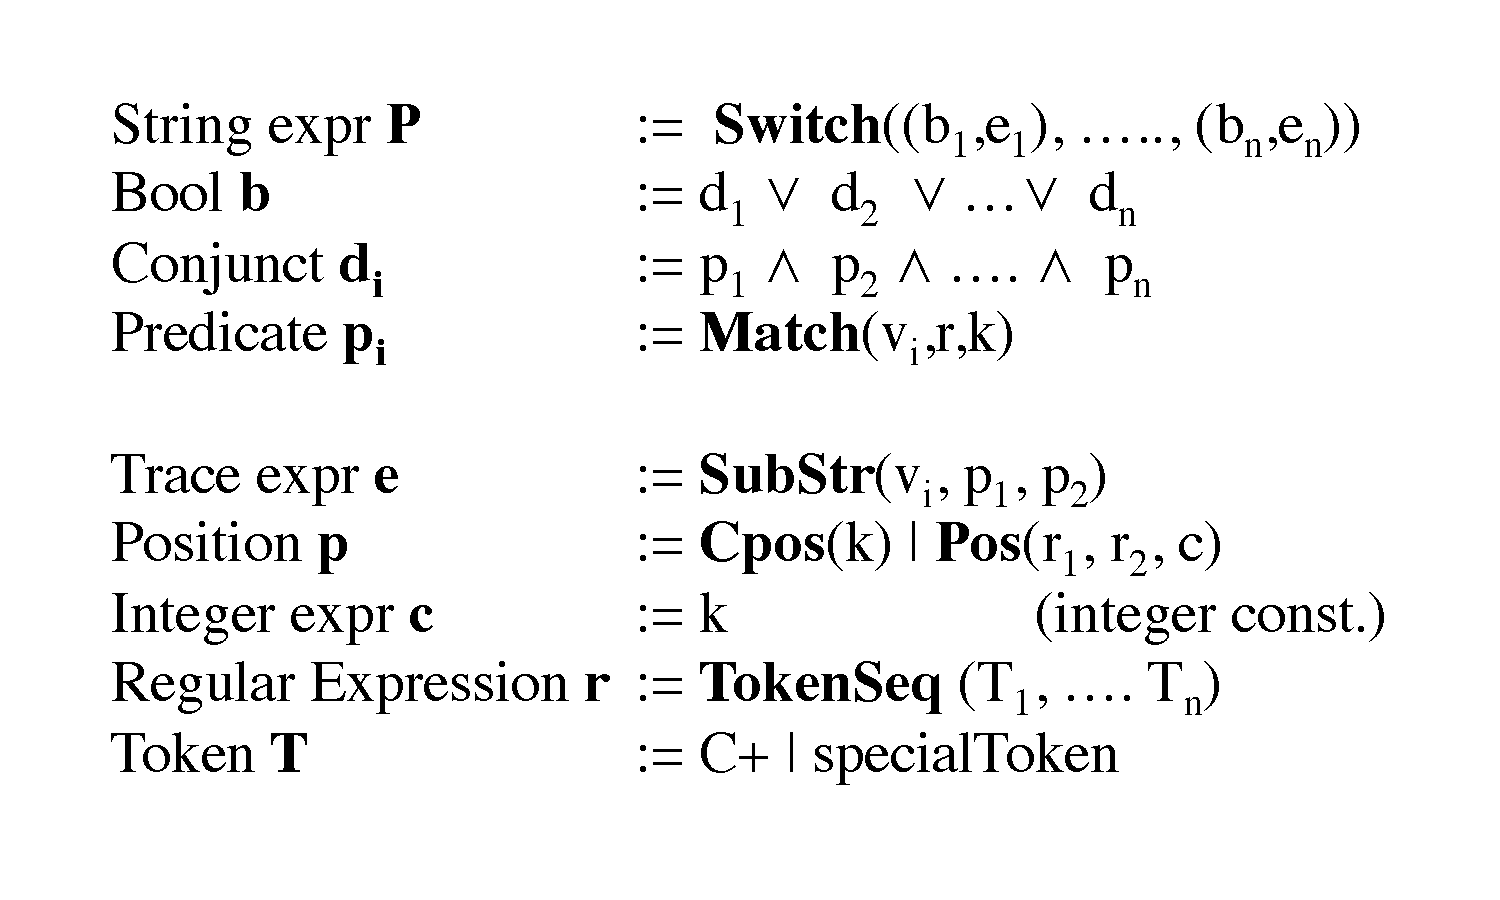
\includegraphics[width=0.4\textwidth]{figs/stringLanguage.pdf}
\caption{Language for learning substring extraction}
\label{fig:language}
\end{figure}


We will first describe the high-level logic of the synthesis technique in ~\cite{Gulwani:2011} which synthesizes simple regular expressions to transform input columns of a desired spreadsheet to a desired output column. We choose to build on top of this technique because of the substantial expressive power of its language at achieving our objective. The details of the basic technique is available in ~\cite{Gulwani:2011}. 

{\bf The Algorithm:}

The main aim of the technique is to learn two sets of information from the given input-output examples --- (a) which string transformation is applicable on a particular input to produce the output, and (b) what is the set of regular expressions that transform the input string to the output string.

From each user-provided input-output example, the set of all expressions from the language (shown in Figure~\ref{fig:language}), that could extract the required output string from that input is computed. If there are multiple input-output examples, the substring extraction rules of the multiple examples are intersected to obtain a more concise set of expressions. If the substring extraction rules cannot be intersected, they are maintained as two disjoint sets, which we shall hereby term as a {\it partitions}. 

Finally, for each disjoint set of extraction rules/regular expressions, a boolean classifier is built in the Disjunctive Normal Form (DNF), to differentiate the examples in one partition to examples in all other partitions. When a new string is given to this tool, the classifier is applied on it to figure out which partition the new input falls into, and the corresponding set of transformation expressions are then applied on it.

{\bf The Language:}

The top level expression of the language is the classifier --- the {\bf Switch}$(b_i,e_i)$ function, which applies the substring expression $e_i$ to the input only if it matches the boolean expression $b_i$. The boolean function is in DNF form and is composed of predicates of the form {\bf Match}$(v_i,r,k)$ , which evaluates to true, iff the input $v_i$ has $k$ occurrences of the regular expression $r$.

The Substring expression {\bf SubStr}$(v_i,p_1,p_2)$, evaluates to the substring between positions $p_1$ and $p_2$ of the string $v_i$. {\bf CPos}$(k)$ denotes the integer position $k$ in the substring. A position expression {\bf pos}$(r_1,r_2,c)$ when applied on a string $s$ evaluates to an integer position $t$ in the subject string $s$ such that $r_1$ matches some suffix $s[0 ..t]$ and $r_2$ matches some prefix of $s[t ... l]$ (where $l$ = Length$(s)$). Also, $t$ is the $c$th such match starting from the left end of the string. If such an position $t$ does not exist in the string, this operator fails. The regular expressions are either just a single token $\tau$, or a token sequence, {\bf TokenSequence}$(\tau_1 .. \tau_n)$, or $\epsilon$ (which matches the empty string). The tokens $\tau$ comprise of a single token to denote alphabetic characters ( referred to as {\it AlphTok}) , one for numeric characters (referred to as {\it NumTok}), and one for each special character. The final result of the application of the {\bf SubStr}$(v_i,p_1,p_2)$ operation yields the output.

We provide a couple of examples to elucidate how this technique works. 

{\bf Example 1}:

Consider, again, the sensor name \texttt{BLDA1R465\_\_ART}. If the desired output is the substring \texttt{ART} can be obtained, among other expressions, by either of the following language transformations :  SubString$(s, $ Cpos$(11)$, Cpos$(14))$, or SubString$(s,$ Pos(UnderscoreToken, {\it AlphTok},$1$), Pos({\it AlphTok},$\epsilon, 1))$.

{\bf Example 2}: 

Suppose the synthesis algorithm has seen two examples \texttt{BLDA1R465\_\_ART}, whose desired output is \texttt{A} at index 3,  and \texttt{BLD\_\_R479\_ART}, whose desired output is \texttt{479}. One of the possible expressions that the synthesis algorithm can come up with is : Switch($(b_1, e_1), (b_2,e_2)$, where $b_1 =$ Match($s$, {\it AlphTok} {\it UnderscoreTok},$1$), $e_1=$ Substring($s$, Cpos(3), Pos({\it AlphTok}, {\it NumTok},1)), and $b_2=$ Match($s$, {\it UnderscoreTok} {\it AlphTok}, 2) and $e_2$ = SubString ($s$, Cpos(6), Cpos(9)).

In general, there can be many expressions in the defined language that can obtain the desired substring, and provide a classifier to specify which types of inputs each type of substring extraction should work on.

%
%{\bf Example:} 
%
%\begin{list}
%\item example 1
%\item example 2
%
%\end{list}

\subsection{Adapting the Language for sensor name qualification}
\label{sec:adapt}

The intuition behind adapting this synthesis technique to our context is that we can independently consider each ({\it tag}) to be a potential output for an inputed string sensor name. If the tag can be applied to qualify a substring of the sensor name, then the output would be the required substring. In all other cases, the output would be $\epsilon$ or the null  string. 

Thus, for each expert-given input-output example\footnote{which in our case is the list of tuples defined in the terminology} and for each tag in the output of that example, we can compute the set of all expressions from the language that could extract the required tag's substring from that sensor name. We then learn a boolean classifier $b_1$such that all tags that are present in the example evaluate their {\bf Switch}($b_1$,$e_1$) condition on this example to True, and all the tags that are not, evaluate theirs to be False. If the {\bf Switch}($b_1$,$e_1$) returns False, then the substring extracted is $\epsilon$, signifying that the tag is not applicable on the sensor name.

If the same tag is present in multiple examples, the tag's new substring extraction expression set is the intersection of it's substring extraction expression sets for each of those examples. This may result in disjoint {\it partitions} of rules for a particular tag. Finally, a boolean classifier is built to differentiate examples of each partition of a tag from all other provided examples. 

However, we run into various challenges if we directly apply this technique to sensor names. We conducted an experiment where we provided examples for sensor names from a building containing 1585 sense points, applying the above-mentioned synthesis technique with no adaptation. The synthesis algorithm applies the tags that it has seen from its existing set of input-output examples on the remaining sensor names. After every run of the algorithm,  on the present set of input-output examples, a new example was chosen at random from the corpus of all sensor names, and a full qualification of it was provided as the next input-output example. Figure~\ref{fig:simpleTokenNoCoverage} shows the result of our experiment.

%% FIX THIS 

We would expect the number of sensor names to have been {\it fully qualified} to increase with each added input-output example. We find this trend up to around 25 examples, after which the synthesis technique started applying erroneous tags to sensor names. At closer inspection, it turns out that the tokens token set used by the regular expressions and the {\bf Match} predicates were not expressive enough to capture the difference of applicability of different tags. 

To illustrate the problem, consider the examples 

{\it Example 1} : \texttt{BLDA4S1831\_STA} : [ (site, \texttt{BLD}, const), (ahu, \texttt{A}, const), (ahuRef,\texttt{4}, var), (supply fan,\texttt{S}, const), (supply fanRef,\texttt{1831}, var), (status point,\texttt{STA},const) ] ; and 

{\it Example 2}: \texttt{BLDA3R5871\_VAV} : [ (site, \texttt{BLD}, const), (ahu, \texttt{A}, const), (ahuRef, \texttt{3}, var), (zone, \texttt{R}, const), (zoneRef, \texttt{5871}, var), (vav, \texttt{VAV}, const) ]

Both these sensor names have the exact same arrangement of numeric and alphabetic characters, and special symbols, and no regular expression used by {\bf Match}$(v_i,r,c)$  would be able to discern between the two. This resulted in erroneous extra tags being applied to sensor names. Hence, we modify the existing language and set of tokens to stay general enough, yet be more expressive. \\

\begin{figure}[h!]
  
  \centering
    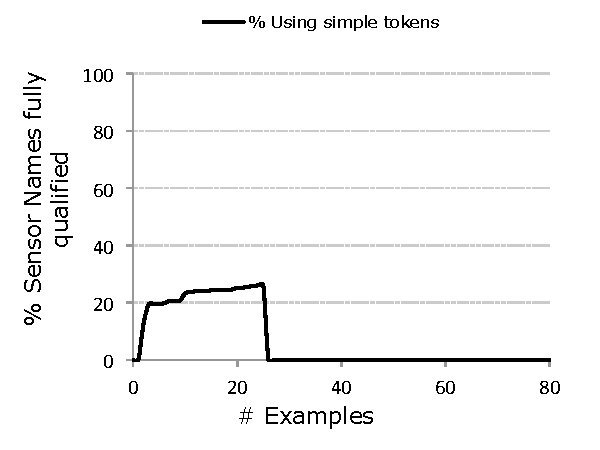
\includegraphics[width=0.40\textwidth]{figs/gulwani-noconverge.pdf}
\caption{Number of sensor names correctly fully qualified with a token set consisting of {\it AlphTok}, {\it NumTok}, {\it SpecialCharToken}}
\label{fig:simpleTokenNoCoverage}
\end{figure}

\subsubsection{Challenges}

Adaptation of the synthesis technique to our context involves certain challenges. First, the number of tags required to fully qualify an entire building might be large, whereas certain tags may be applicable on a very limited number of sensor names. In such a case, the classifiers and the corresponding regular expressions $r$ should be expressive enough to differentiate a small group of sensor names from the remaining. One way to increase the expressive power of the regular expressions $r$ is to have certain building-specific tokens in addition to the normal alphabetic, numeric and special character tokens. Different conventions of sensor naming from building to building precludes us from having an a priori set of special tokens.

Second, a building may have 1000s of sensor points, making visual inspection of correctness of sensor name qualification very hard. Hence, wrong application of a tag to a particular sensor name is likely to go unnoticed. We mitigate this by being more conservative with the boolean classifier $b$ in the top level {\bf Switch} operator. \\

% incremental intersection . 

Below, we list four techniques that augment the basic language shown in Figure~\ref{fig:language} to enable correct classification of 

\subsubsection{Token Set}

In our last example we showed earlier, the set of regular expressions were not powerful enough to differentiate between two sensor names if we use one token for alphabetic character class, one for the numeric character class, and one for each special symbol. Also, the set of tokens which make sense in the context of sensor names vary across buildings, and across vendors.

%An alternative would be to use a different token for every individual alphabet, which would have been able to discern between the two sensor names. However, this makes the set of regular expressions obtained very specific to this particular building. 
%
%One building in our testbed had variable values which consisted of a combination of alphabets and numerals , e.g \texttt{BLD2.PWR.CL42A.REACTIVE POWER}, which describes that is a sensor point in building \texttt{BLD2}, that senses the reactive power of the power meter \texttt{CL42A}, which is a variable value (since it is sensor-specific). This building also had other power meters which had identifications of the form \texttt{DM12}, etc. Using a token for each different alphabetic character would not be able to express both of them as outputs to the {\bf power meter Ref} tag without multiple examples.

To solve this, we utilize the constant tag values in the examples provided by the expert as special tokens for the regular expressions to be generated from that example, in addition to the normal tokens described above. Thus, the sensor name \texttt{BLDA1R465\_\_ART}\footnote{whose output example provided by the expert was (site, \texttt{BLD}, const), (ahu, \texttt{A}, const), (ahuRef,\texttt{1}, var), (zone,\texttt{R}, const), (zoneRef, \texttt{465}, var), (zone air temp sensor, \texttt{ART}, const). } is treated as a set of tokens [ (BLD)(A)[{\it NumTok}](R)[{\it NumTok}]+ {\it UnderscoreTok} {\it UnderscoreTok} (ART) ].


Similarly, suppose the input-output example provided by an expert for a sensor name \texttt{BLD2.PWR.CL42A.REACTIVE POWER} is [ (site,\texttt{BLD2},const), (power meter, \texttt{PWR},const), (power meterRef,\texttt{CL42A},var), (reactive power, \texttt{REACTIVE POWER}, const) ]   
This string is treated as a combination of tokens [ (BLD2) {\it dotTok} (PWR) {\it dotTok} [{\it AlphTok}]+[{\it NumTok}]+[{\it AlphTok}] {\it dotTok} (REACTIVE POWER) ]. 

Note that this provides enough expressibility for the regular expressions to differentiate between the two inputs \texttt{BLDA4S1831\_STA}, and  \texttt{BLDA3R5871\_VAV} from the user, which was impossible using only the normal tokens. \\

\subsubsection{Splitting constant tags}

In order to improve the efficiency of the classifier, we consider a tag having multiple constant values, as different tags. For instance, in our test building, an {\it exhaust fan} tag was applicable either as the constant characters \texttt{E} or the constant character \texttt{EF}. Note that the index of the various other tag's values in a sensor name change depending on which of the constant value appears, rendering previously learnt Cpos(k) operators useless. 

We treat the same tags which maybe represented by two different constant string to be two different tags altogether. This enables a richer intersection set when tag outputs from the expert-given examples are combined. 

\subsubsection{Modifying Boolean Classifiers}

Since manual inspection of the qualification of all the points is not feasible, we take steps to strengthen the boolean classifiers corresponding to each tag. We implement different strategies for tags that have constant and variable values.

If a tag has a constant value, we ensure that each boolean clause $d$ in the DNF expression used by the {\bf Switch} operator has a {\bf Match}($s$, constTagValue, $k$) as the first conjunct $p_1$ , where $k$ is the number of times the constant value appears in the examples. This ensures that if a tag is evaluated to be applicable on a string, the constant substring does exist in the string.

Next, in cases where a tag which has a variable value, and is a reference to another tag with a constant value which is applicable on the same string, we mandate that the constant tag also have been deemed applicable on the same sensor name. For instance, in the example \texttt{BLDA1465\_ART}, the tag {\it zoneRef} whose value is to \texttt{465} has a reference to the {\it zone} tag, which has a constant value. Thus, we would only evaluate the {\bf Match} expressions for {\it zoneRef} iff the the {\bf Match} condition for the {\it zone} tag has also evaluated to True. \\




\subsubsection{Modifying Matching expression}

To make the classifiers more general, so that regular expressions learnt for one building may be applicable to sensor names of other buildings with a similar naming convention, we augment the language to include 

Predicate {\bf $b_i$} $:=$ {\bf Match}$(v_i, r, k) |$  {\bf CMatch}$(v_i, r , k)$,

where  {\bf CMatch}$(v_i, r , k)$ evaluates to true iff the regular expression is satisfied at position equal to $k$. 

Suppose, from the technique encounters only one example \texttt{BLDA1R465\_\_ART} , and for the {\it zone temp sensor} tag learns a classifier $b_1$ =  {\bf Match}$(s,$(ART),1) for application of the {\it zone temp sensor} tag. Now, if another building was abbreviated as \texttt{ART}, and the synthesis technique encountered a sensor name of the form \texttt{ARTA2R354\_\_ART}, the classifier would fail to apply the {\it zone temp sensor} tag because there are two matches to the regular expression (ART) in the string, and  {\bf Match}$(s,$(ART),1) would evaluate to false.

Whenever possible, we apply {\bf CMatch} before {\bf Match} expressions while generating classifiers mitigates some of the issues which arise from using the previously defined {\bf Match} token.



\section{Evaluation of Learning By Example}
\label{sec:eval}

In this section, we guage the effectiveness of our learning by example technique by evaluating the number of examples required to qualify labels in two large commercial buildings. 

\subsection{Testbed}

We manually generated ground truth data for all the points in two buildings whose building management system was installed by different vendors. Building $1$ has 1586 sensor points and was built in the 1990s. Building $2$ was built in the 2000s and has 2551 sense points. The label characteristics of the two buildings are shown in Figure~\ref{fig:buildingLabelCharacteristics}. 

Figure~\ref{fig:labelFreq} shows that in  these two buildings, a few tags (about 20 in each building) frequently appear in a lot of sensor names. This is pretty common in commercial buildings, where a majority of the points are related to zone or room information. For instance, Building $1$, has a room setpoint sensor, an airflow sensor and temperature sensor for each of its more than 200 rooms. For each of these points, the {\it zone} and {\it zoneRef} tags are applicable because there exist characters which specify that it is a zone and it zone number. These most frequent tags also fully qualify a large number of the sensor names in both buildings. As shown in Figure ~\ref{fig:pointCDF},  learning proper classifiers and qualifications for about 20 labels could yield a full qualification for 70-80\% of the sensor names in both these buildings.

The distribution frequency of applicable tags also has a long tail. These comprise of tags for building specific sensors, alarms or status variables. Thus, one of the main objectives of the learning algorithm is that it does not learn wrong classifiers for tags based on sensor names that fall in this long tail.

\begin{figure}[h!]]
\centering
	\begin{subfigure}{0.40\textwidth}
                \centering
		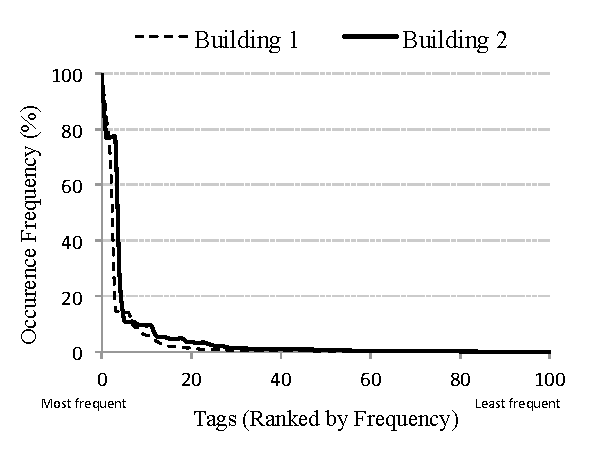
\includegraphics[width=\textwidth]{./figs/pointOccuranceFreq.pdf}
                \caption{Percentage of sensor names each tag appears in. The x-axis is sorted according to the frequency of occurrence of a label}
                \label{fig:labelFreq}
	\end{subfigure}
	\begin{subfigure}{0.40\textwidth}
                \centering
		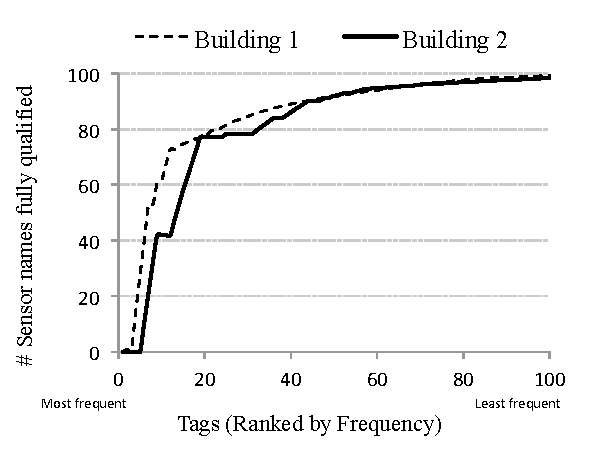
\includegraphics[width=\textwidth]{./figs/pointCDF.pdf}
                \caption{Percentage of sensor names fully qualified by the highest ranking tags. A point ($x$,$y$) indicates that $y$ sensor names could be fully qualified by using labels ranked $1$ ... $x$}
                \label{fig:pointCDF}
	\end{subfigure}
\caption{Characteristics of tag application from two buildings we generated complete ground-truth data for, to test our learning technique}
\label{fig:buildingLabelCharacteristics}
\end{figure}


\begin{figure}[h!]
\centering
	\begin{subfigure}{0.40\textwidth}
                \centering
		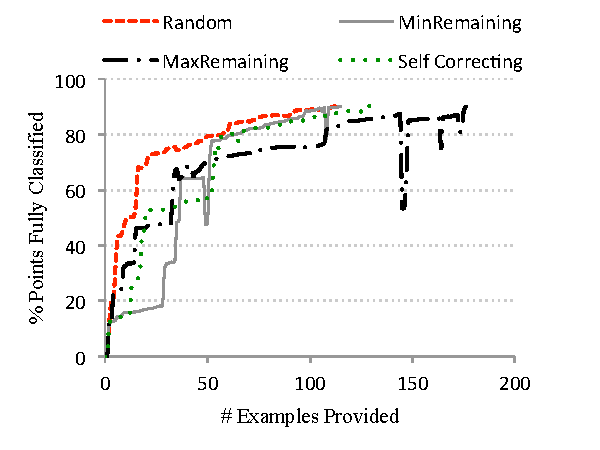
\includegraphics[width=\textwidth]{./figs/soda-active-learning.pdf}
                \caption{Building 1}
                \label{fig:active-learning-soda}
	\end{subfigure}
	\begin{subfigure}{0.40\textwidth}
                \centering
		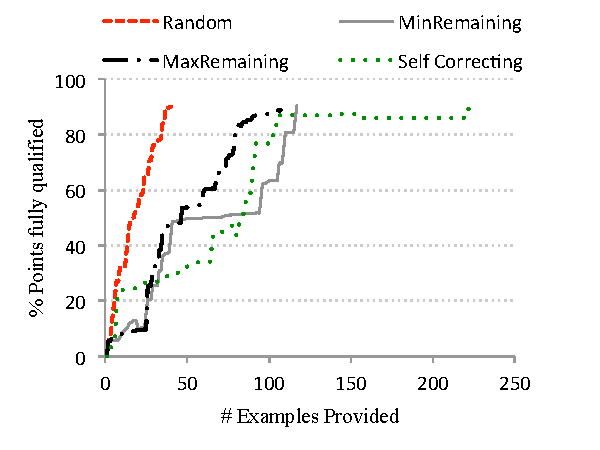
\includegraphics[width=\textwidth]{./figs/sdh-active-learning.pdf}
                \caption{Building 2}
                \label{fig:active-learning-sdh}
	\end{subfigure}
\caption{The number of examples required to fully qualify 90\% of sensor names in two buildings. The {\it Random} generator achieves 70\% full sensor name qualification within 25 examples for Building $1$ and 27 examples for Building $2$.}
\label{fig:active-learning}
\end{figure}


\subsection{Choosing the Next Example}


The large number of sensors in a building pose a challenge in selecting the next example to present to the expert. First, the expert might not always be able to browse through all sensor points to check correct qualification. Also, an expert might visually not be able to discern which points would add the most amount of information to the learning process. 

We implemented four different generators to evaluate which example should be provided next to the expert:

{\it Random:} This generator just finds at random the next example to present to the expert. While choosing the example, the random algorithm chooses among the set of sensor names which it feels it has not been able to fully qualify.  

{\it MinRemaining :} This generator chooses the example, that according to our tool, has the minimum string length left to qualify. The intuition behind this is to gain more concrete knowledge about a small number of labels.

{\it MaxRemaining :} This chooses the example, that the learning technique feels has the maximum string length left to qualify. These examples would help the learning technique gain coverage over the space of unseen labels. The more labels the learning technique knows, the more sensor name information it will be able to qualify.

{\it Self Correcting :} There are some sensor names where the learning algorithm can itself figure out that it has incorrectly qualified a sensor name. There can be three such indicators. First, for a sensor name which has matched its boolean classifier, but none of its set of {\bf SubString} regular expressions is applicable. Second, if the sensor name has been qualified with labels that overlap over the same substring region. Third, the learning algorithm can get a notion of the qualification uncertainty of a sensor name, if its (tag, value) tuples change drastically when a new example has been added. This generator gives the expert the examples that satisfy the most number of these three criteria. Once, none of the points satisfy these criteria, this generator defaults to the MinRemaining generator.

{\bf Experiment :}

We wrote a script that automatically gave the synthesis tool the example that it asked for, and compared the qualifications for all sensor names outputted by it after the processing the example,  to the ground truth. We ran one experiment for each of the generators. We terminated when the number of correct full sensor qualifications reached 90\%. A full qualification of a sensor name into (tag, value) tuples is correct if (a) the correct tags were applied on it and  obtained the correct values corresponding to each tag, (b) No extra incorrect tag was applied to the sensor name, and (c) the tags were able to fully qualify every alphanumeric character of the sensor name.


{\bf Results : }

Figures ~\ref{fig:active-learning} show the results of the four generators on the two buildings. The \emph{Random} generator took the least number of examples to achieve full qualification of 70\% of the sensor names, achieving it much quicker than the others. The reason for this is due to the long tail of the label distribution of tag names (  Figure~\ref{fig:labelFreq}). The top 20 most occurring tags, by themselves, can fully qualify about the majority of the sensor names. A random generator has a high probability of finding one of these points, thus acquainting itself more quickly of the most frequently occurring labels. Neither of the other three classifiers is able to achieve that. They get stuck trying to learn regular expressions from sensors with obscure tags (\emph{MinRemaining}), or trying to cover more labels by first qualifying sensors which have been least qualified, which comprise mainly of sensor names which are inconsistently named (\emph{MaxRemaining}), or by choosing form the set of ill-formed sensor names, which would indicate errors to the learning algorithm (\emph{Self-Correcting}).

The number of example reach 90\% qualification, is however, similar across all the generators. Going from 70\% to 90\% takes about 85 extra examples for the {\it Random} generator. The process is much smoother for Building $2$ which has better defined point names, and fewer inconsistent or incomplete point names.

{\bf Conlusion :}

The results show that a {\it Random} approach while seeking the next sensor name to get an example of, leads the synthesis technique to quickly accurately fully qualify a large fraction of the sensor names (70-80\%). This result may also be generalizable to other commercial buildings for which zone-related sensors comprise a major fraction. However, going from 70\% full qualification to 90\% full qualification takes a long time, as these point comprise of tags that are infrequent.

\begin{figure}[h!]
\centering
	\begin{subfigure}{0.40\textwidth}
                \centering
		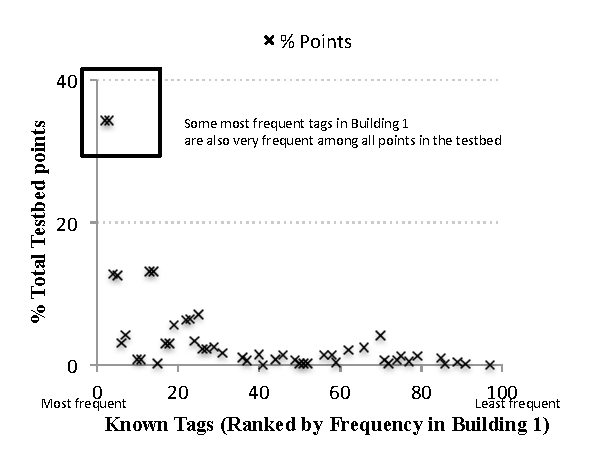
\includegraphics[width=\textwidth]{./figs/campusWideStats-point.pdf}
                \caption{Occurrence frequency of tags learnt from Building $1$ to the other 55 buildings in our testbed. The most common tags in Building $1$ ( e.g {\it zoneRef} ) are also applicable to around 35\% of all the sensor in the testbed.}
                \label{fig:campusWideStats-build}
	\end{subfigure}
	\begin{subfigure}{0.40\textwidth}
                \centering
		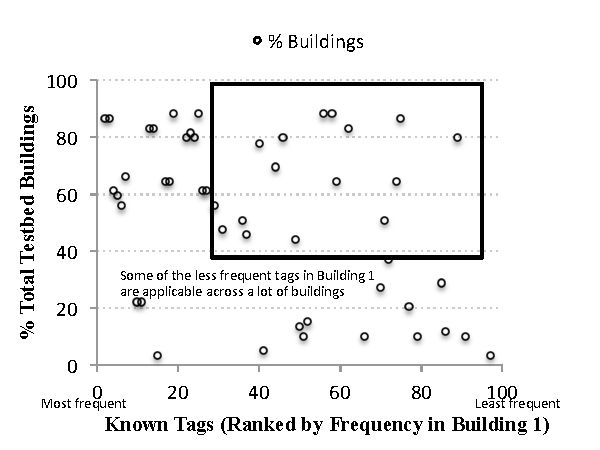
\includegraphics[width=\textwidth]{./figs/campusWideStats-build.pdf}
                \caption{Occurrence frequency of a tag across buildings. Even though some tags are less frequent (e.g {\it Chilled water temp} tag), they do occur across 60-80\% of the buildings. }
                \label{fig:campusWideStats-build}
	\end{subfigure}
\caption{Applicability of existing tags learnt from Building $1$ to the remaining 55 buildings in out testbed. Missing values corresponding to an x-axis value indicates that the particular tag did not appear in any of the other buildings}
\label{fig:campusWideStats}
\end{figure}


\begin{figure*}[ht!]
\centering
	\begin{subfigure}{0.4\textwidth}
                \centering
		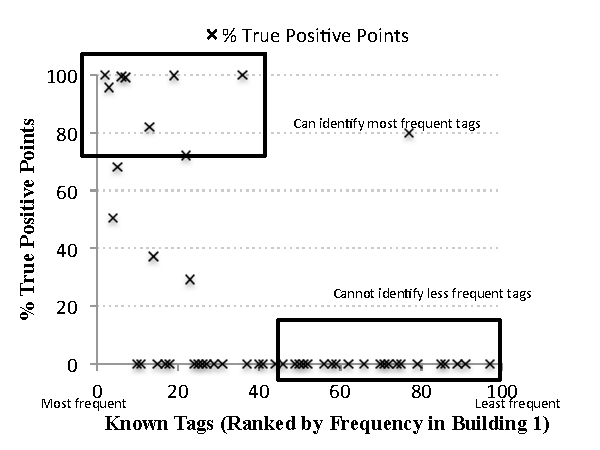
\includegraphics[width=\textwidth]{./figs/recallCampusWide-point-50.pdf}
                \caption{Applying Regular expressions obtained after 50\% full qualification of Building $1$ by {\bf Random}}
		\label{fig:point50}
	\end{subfigure}
	\begin{subfigure}{0.4\textwidth}
                \centering
		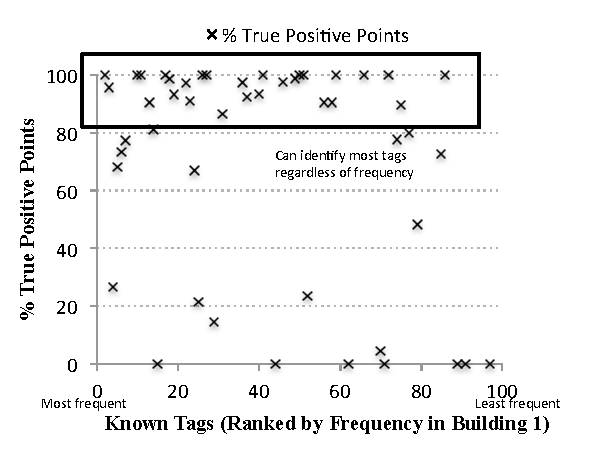
\includegraphics[width=\textwidth]{./figs/recallCampusWide-point-90.pdf}
                \caption{Applying Regular expressions obtained after 90\% full qualification of Building $1$ by {\bf Random}}
		\label{fig:point90}
	\end{subfigure}
	\begin{subfigure}{0.4\textwidth}
                \centering
		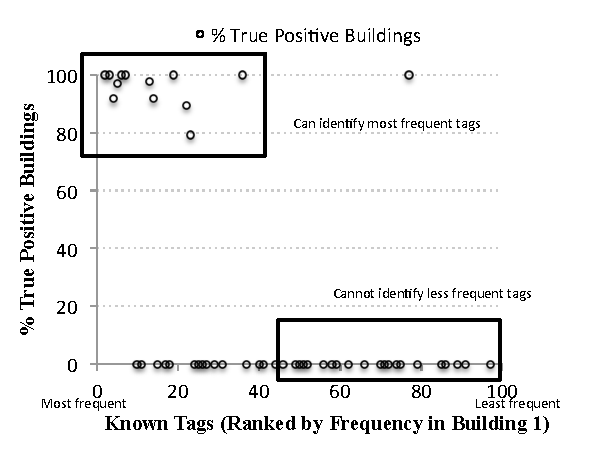
\includegraphics[width=\textwidth]{./figs/recallCampusWide-build-50.pdf}
                \caption{Applying Regular expressions obtained after 50\% full qualification of Building $1$ by {\bf Random}}
		\label{fig:build50}
	\end{subfigure}
	\begin{subfigure}{0.4\textwidth}
                \centering
		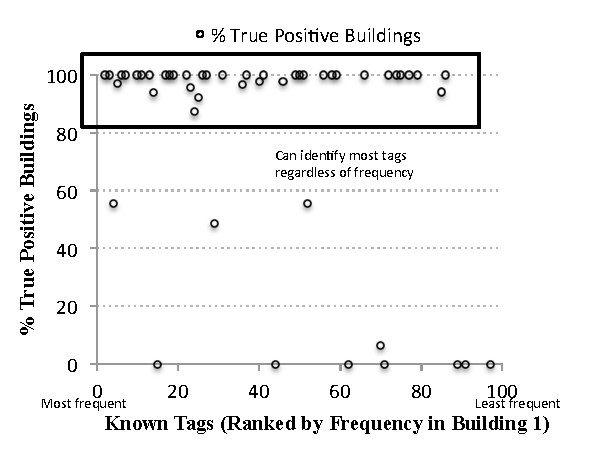
\includegraphics[width=\textwidth]{./figs/recallCampusWide-build-90.pdf}
                \caption{Applying Regular expressions obtained after 90\% full qualification of Building $1$ by {\bf Random}}
		\label{fig:build90}
	\end{subfigure}


\caption{Figure showing that while the {\it Random} generator can quickly obtain full qualification of 70\% of a particular building's point names, it is less effective at learning the regular expressions for lower frequency tags, which may also be applicable across a lot of Buildings (Figure~\ref{fig:campusWideStats-build}). However, if a lot more examples are given, such that the {\it Random} generator can fully qualify 90\% of Building $1$'s point names (about 110), it get obtain good regular expression for the infrequent tags as well, and be able to correctly apply them in an unknown building.}
\label{fig:recallCampuswide}
\end{figure*}


\subsection{Applying Learnt Expressions to unknown buildings}

%This Figure shows the efficacy of using the regular expressions learned on Building $1$ in qualifying point names with similar tags in other buildings, for three different set of expressions obtained from our language after applying the {\bf Random} example generator in the previous experiment until it had achieved 50, 70 and 90\% full qualifications of sensor names in Building $1$. The x-axis are the tags ordered by their frequency of occurence in Building $1$. The primary y-axis shows the true positive rate of identifying a particular tag in the point names in other buildings as compared to our ground truth data. The secondary y-axis shows the true positive rate rate of identifying a tag in a different building as compared to our ground truth data



%
%\begin{figure}[h!]
%  
%  \centering
%    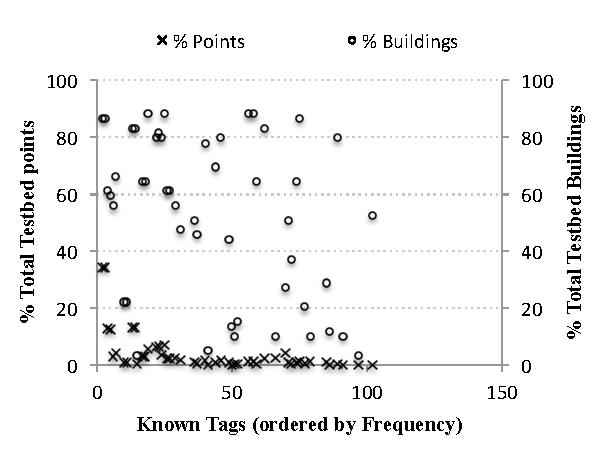
\includegraphics[width=0.5\textwidth]{figs/campusWideStats.pdf}
%\caption{Applicability of the tags learnt from Building $1$ to other buildings in our testbed.A tag is applicable to another point name if it either is the same constant value as encountered in Building $1$, or if the point name has a variable substring which could be qualified using the same tags as found in Building $1$.  The x-axis are the tags ordered by their frequency of occurence in Building $1$. If there is no value corresponding to a particular value on the x-axis, it indicates that the particular tag was not applicable to any other building. The primary y-axis shows the percentage of total point names in the remaining buildings the same tags are applicable to. The secondary y-axis shows the percentage of the number of buildings a particular tag may be used to qualify a sensor point of.  }
%\label{fig:campusWideStats}
%\end{figure}




One of the major goals of learning from examples provided by an expert is that the learnt regular expressions may be applicable to other buildings which have similar naming conventions. In this section, we evaluate the efficacy of the regular expressions learnt on Building $1$ of our testbed with the remaining 55 buildings on campus, each of whose building management system sensors was commissioned by the same vendor. As mentioned before, the remaining buildings comprise about 16,000 sensor points.

{\bf Testbed for experiment:}

Figure~\ref{fig:campusWideStats} shows the applicability of tags learnt from Building $1$ to the remaining buildings. Tags which were most frequent in Building $1$ such as {\it zone, zoneRef} and {\it ahuRef}, were also widely applicable throughout other buildings. This is expected because all these buildings are commercial offices, with a large number of zone, and a set of points associated with each zone. There are also a few tags which are infrequent in a particular building, but applicable across all buildings, e.g the {\it return water temp} tag or the {\it outside air temp} tag. Thus, fully qualifying even one building has the potential to yield regular expressions that can then be propagated across buildings.

{\bf Experiment:}
It was impractical to ground truth all the buildings and its 16,000 sensor points for our experiment. Hence, we hand wrote regular expressions to the best of our efforts to qualify sensor names in those buildings. It is this manual qualification data that we treat as ground truth in the our experiment. We run three experiments, where we use the regular expressions obtained after 50 and 90\% full qualification results obtained by the {\it Random} process in the previous experiment(see Figure~\ref{fig:active-learning-soda}).While running these expressions on a different building, we just replaced the token corresponding to the tag {\it site} to the building-specific {\it site}  token. 

{\bf Results:}

Figure~\ref{fig:recallCampuswide} shows the true-positive rate of the tags applied to the 15000 sensor names across 55 buildings, based for each tag based on our ground truth data. The true positive rate indicates that the required tag was correctly applied where it was applicable, and it was able to qualify the correct substring from the corresponding sensor name. 

There is direct effort-applicability correlation. The more fully qualified a particular building is, the more tag applicability expressions are learnt. When enough examples were provided such that Building $1$ had correctly fully qualified only 50\% of the sensor names, the synthesis technique had either not encountered a lot of the lesser frequent tags, or did not have enough examples to build a robust classifier, leaving the regular expression set unable to discover the same tags in the remaining point names(Figure~\ref{fig:point50}). Also, this trend was true across buildings, where the inferior set of regular expressions was not able to properly apply the lower frequency tags on any building (Figure~\ref{fig:build50}).

However, when enough examples for 90\% full qualification was provided ( 110 examples for Building $1$), the synthesis algorithm was able to correctly identify and qualify a lot of the tags which had a low frequency in Building $1$. This is due to the exhaustive list of regular expressions it had to generate to fully qualify the obscure point names in Building $1$ in order to get a 90\% accurate full qualification. 

%Thus, even though a random generator can quickly label most of the sensor names in a particular building, it may not be able to transfer all of the tags which can be propagated to other buildings. Herein lies a tradeoff between choosing the Random generator to show the expert new examples, or showing the user examples with knowledge of a larger set of buildings in mind. 

Some of the tags could not be applicable to other buildings, because they use different constant values for the same tag name. For instance, the {\it exhaust fan} tag is specified in certain buildings as \texttt{EF}, wheras in Building $1$ it was specified as \texttt{E}. Also, certain tags which extract variable values (the {\it zoneRef} tag) face some challenges when scaling across buildings. 

{\bf Conclusion:}

We conclude that using the {\it Random} generator to ask for the next example, the number of examples required to qualify a large fraction (e.g 70\%) of a commercial building's point names might be few ( 24 example for Building $1$ ). During the process, though, the generator does not learn the expressions needed to qualify the lower frequency tags, a lot of which are common across buildings. 

Trying to accurate fully qualify 90\% of a building's point names forces the synthesis algorithm to encounter a encounter the less frequent tag names ,and hence it is able to apply these lower frequency tags when they apply across buildings. However, Building $1$ in our testbed required about 85 more examples to reach from a full qualification of 70\% of the sensor to a full qualification of 90\% of the sensors. 
%
%Our result displays the promise of program synthesis in learning the metadata structure of buildings and propagating the learnt structure on to other buildings with a similar metadata structure. There are two specific observations that we would want to make about the applicability of this synthesis technique across other sets of buildings. 
%
%First, as mentioned earlier, our testbed contains mainly commercial buildings have a large number of rooms/zones and zone related sensors. Thus learning the pattern for one zone may allow the regular expressions to propagate to similar sensors to all the other zones in the building. This, howver, may not hold true for industrial buildings, where large collection of sensors all of which serve similar subsystems  may be non-existent.
%
%Secondly, we found an interesting  between the effort put in to augment the 
%
%\begin{figure*}[ht!]
%\centering
%	\begin{subfigure}{0.4\textwidth}
%                \centering
%		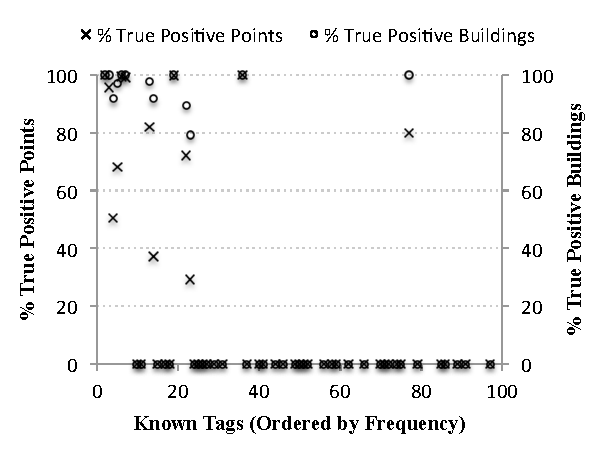
\includegraphics[width=\textwidth]{./figs/recallCampusWide-50.pdf}
%                \caption{Regular expressions obtained after 50\% full qualification by {\bf Random}}
%		\label{fig:full50}
%	\end{subfigure}
%	\begin{subfigure}{0.4\textwidth}
%                \centering
%		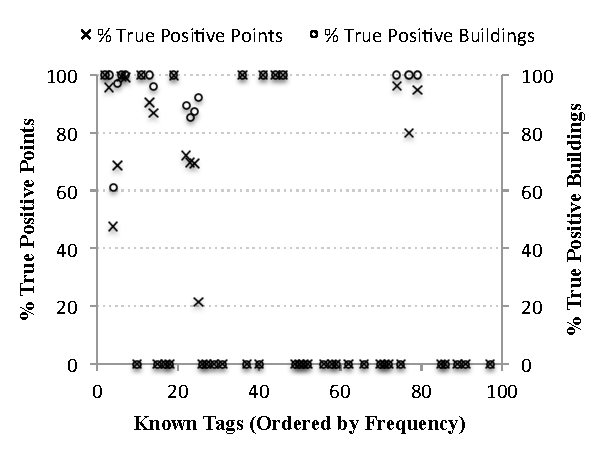
\includegraphics[width=\textwidth]{./figs/recallCampusWide-70.pdf}
%                \caption{Regular expressions obtained after 70\% full qualification by {\bf Random}}
%		\label{fig:full70}
%	\end{subfigure}
%	\begin{subfigure}{0.4\textwidth}
%                \centering
%		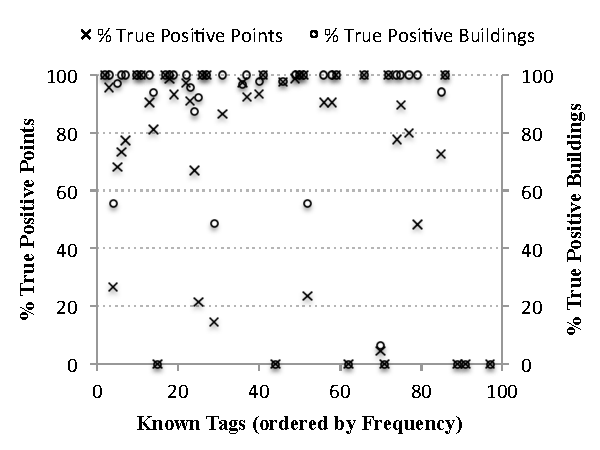
\includegraphics[width=\textwidth]{./figs/recallCampusWide-90.pdf}
%                \caption{Regular expressions obtained after 90\% full qualification by {\bf Random}}
%		\label{fig:full90}
%	\end{subfigure}
%\caption{This Figure shows the efficacy of using the regular expressions learned on Building $1$ in qualifying point names with similar tags in other buildings, for three different set of expressions obtained from our language after applying the {\bf Random} example generator in the previous experiment until it had achieved 50, 70 and 90\% full qualifications of sensor names in Building $1$. The x-axis are the tags ordered by their frequency of occurence in Building $1$. The primary y-axis shows the true positive rate of identifying a particular tag in the point names in other buildings as compared to our ground truth data. The secondary y-axis shows the true positive rate rate of identifying a tag in a different building as compared to our ground truth data.}
%\label{fig:recallCampuswide}
%\end{figure*}

%
%\begin{figure}[h!]
%\centering
%	\begin{subfigure}{0.48\textwidth}
%                \centering
%		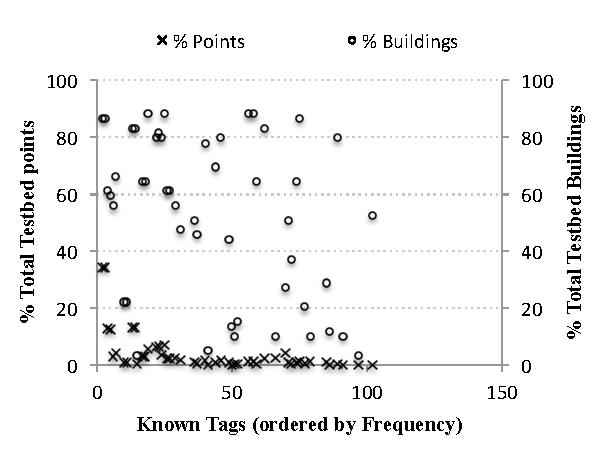
\includegraphics[width=\textwidth]{./figs/campusWideStats.pdf}
%                \caption{Building 1}
%                \label{fig:campusWideStats}
%	\end{subfigure}
%	\begin{subfigure}{0.48\textwidth}
%                \centering
%		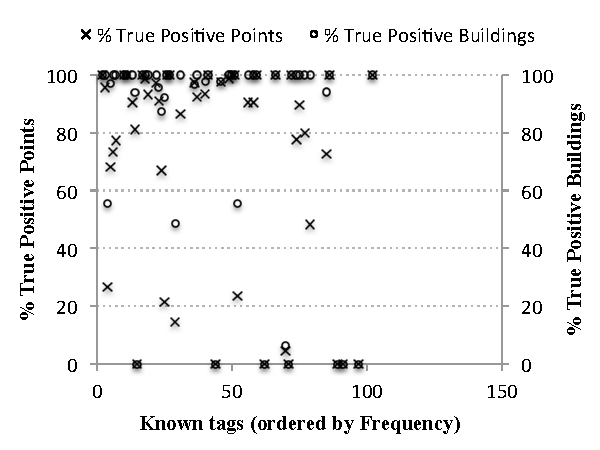
\includegraphics[width=\textwidth]{./figs/recallCampusWide.pdf}
%                \caption{Building 2}
%                \label{fig:recallCampusWide}
%	\end{subfigure}
%\caption{The number of examples required to fully qualify 70\% of sensor names in two buildings}
%\label{fig:active-learning}
%\end{figure}









